\documentclass[11pt,border=4pt]{standalone}
\usepackage{amsmath,amssymb,bm,mathtools}
\usepackage[fontset=fandol]{ctex}
\usepackage{tikz}
\usetikzlibrary{arrows.meta,calc,patterns,angles,quotes,decorations.markings,decorations.pathmorphing}
\newcommand{\dd}{\mathop{}\!\mathrm d}
\newcommand{\e}{\mathrm e}
\tikzset{axis/.style={->,>=Stealth,line width=.45pt},world/.style={line width=.8pt},flow/.style={->,>=Stealth,line width=.7pt},ray/.style={->,>=Stealth,line width=.7pt},guide/.style={dashed,line width=.35pt},aux/.style={dashed,line width=.35pt},dim/.style={<->,>=Stealth,line width=.35pt},every node/.style={font=\small},force/.style={->,>=Stealth,very thick},gas/.style={fill=blue!7}}
\begin{document}
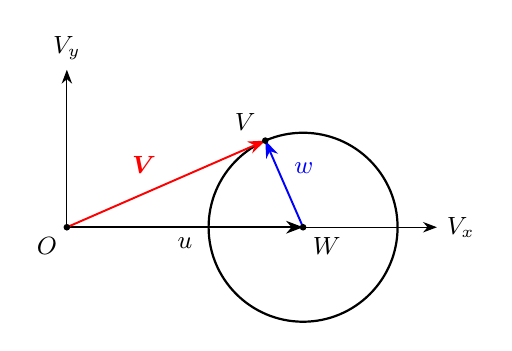
\begin{tikzpicture}
\coordinate(O)at(0,0);\coordinate(W)at(3,0);\coordinate(V)at(2.52,1.1);
\draw[axis](0,0)--(4.7,0)node[right]{$V_x$};
\draw[axis](0,0)--(0,2)node[above]{$V_y$};
\draw[world](W)circle(1.2);\draw[flow](O)--(W)node[midway,below]{$u$};
\draw[flow,blue](W)--(V)node[midway,above right]{$w$};
\draw[flow,red](O)--(V)node[midway,above left]{$\bm V$};
\fill(O)circle(1.2pt)node[below left]{$O$};
\fill(W)circle(1.2pt)node[below right]{$W$};
\fill(V)circle(1.2pt)node[above left]{$V$};
\end{tikzpicture}
\end{document}
